% -*- latex -*-
% FILE: "/home/evmik/jobs/wm/2012_spring_Analog_Electronics_252/final_exam/questions/opamp_adder.tex"
% LAST MODIFICATION: "Mon, 30 Apr 2012 15:45:04 -0400 (evmik)"
% (C) 2011 by Eugeniy Mikhailov, <evgmik@gmail.com>
% $Id:$

\question{}
	Consider the circuit shown below \\
	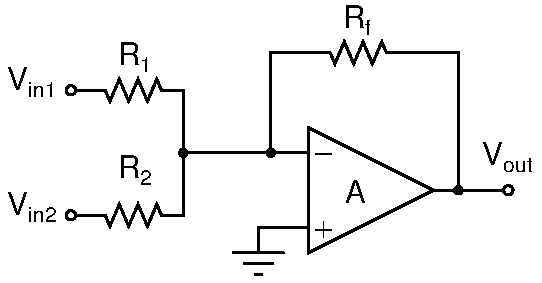
\includegraphics[height=1in]{./schematics/summing_inv_ampl}\\
	The open loop gain $A=\infty$.
	\begin{parts}
		\part[10]
		Derive the expression for the output voltage $V_{out}$, in terms of
		$V_{in1}$, $V_{in2}$, $R_1$, $R_2$, and  $R_f$. Note that $R_1 \neq R_2$.

		\vskip 2.5in
		$V_{out}=$
		\part[3]
		If a power supply provides $\pm15$~V to the amplifier, and $R_f/R_1=2$,
		$R_f/R_2=3$, $V_{in1}=V_{in2}=4$~V. What is the
		output voltage?

		\vskip 2.0in
		$V_{out}=$
		\part[2]
		Same as above but $V_{in1}=1$~V, $V_{in2}=-1$~V.

		\vskip 1.0in
		$V_{out}=$
	\end{parts}
	\pagebreak

